% Chapter Template

\chapter{Ensayos y resultados} % Main chapter title

\label{Chapter4} % Change X to a consecutive number; for referencing this chapter elsewhere, use \ref{ChapterX}

%----------------------------------------------------------------------------------------
En este capítulo se muestran los principales ensayos realizados y sus resultados, para verificar el cumplimiento de los requisitos. Además, se incluye un caso de uso completo.

%----------------------------------------------------------------------------------------
%	SECTION 1
%----------------------------------------------------------------------------------------

\section{Pruebas unitarias}
\label{sec:pruebasUnitarias}

\subsection{Calibración del electrodo}

Para la validación del proceso de calibración del electrodo se utilizó el banco de pruebas que muestra la figura         , y se procedió a realizar el proceso de calibración. La tabla \ref{tab:ensayoCalibracion} muestra las mediciones correspondientes a la diferencia de potencial entregada por módulo pH4502C y al valor leído por el ADC para cada unos de los valores de los \textit{buffers}, en un ambiente con temperatura de 25 °C.

\begin{table}[h]
	\centering
	\caption[Resultados calibración]{Resultados obtenidos durante el proceso de calibración}
	\begin{tabular}{l c c }    
		\toprule
		\textbf{\textit{Buffer} [pH]} & \textbf{Salida pH4602C [V] }	&    \textbf{Lectura ADC}  \\
		\midrule
		4 	& 2,635 \% & 3050 \\		
		7	& 2,172 \% & 2455 \\
		10	& 1,877 \% & 2120 \\
		\bottomrule
		\hline
	\end{tabular}
	\label{tab:ensayoCalibracion}
\end{table}

A partir de los datos obtenidos, se puede graficar la recta de ajuste que relaciona el valor de pH con el valor de medido por el ADC, como se muestra en la figura \ref{fig:rectaADC}. Los valores de pendiente y ordenada al origen calculados en el ESP32 fueron visualizados por el monitor serial, y se obtuvo -0,0063 para el valor de la pendiente m, y 22,98 para el valor de la ordenada al origen b. 

\begin{figure}[htbp]
	\centering
	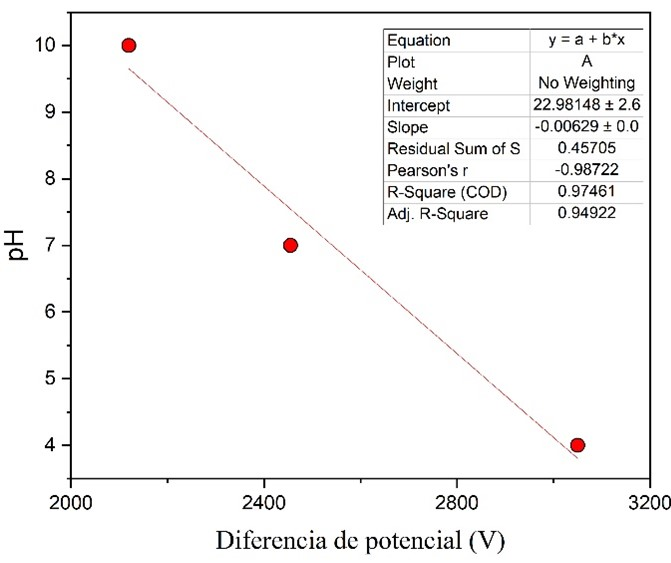
\includegraphics[width=0.7\textwidth]{./Figures/rectaADC.jpg}
	\caption{Relación entre el pH y el valor convertido por el ADC.}
	\label{fig:rectaADC}
\end{figure}

Luego de repetir el ensayo, se obtuvo que el error en la medición del potencial de salida del módulo pH4502C es de +/- 1 mV y luego de la conversión a pH el error es de +/- 0,1 pH a temperatura ambiente. 

\subsection{Calibración del volumen inyectado por la bomba}

Banco de prueba y resultados


\section{Validación y verificación}
\label{sec:validacionVerificacion}